\section{Introduction}
\label{sec:intro}

Evaluation of dialogue systems is still an open question. Existing
automatic evaluation metrics for chitchat systems are similar to those for 
other text generation tasks (e.g. machine translation \citep{papineni-etal-2002-bleu}, question-answering \citep{rajpurkar-etal-2016-squad}, 
summarization \citep{lin-2004-rouge}), which depends on calculating word overlaps with 
ground truth reference responses. 
However, for chitchat tasks, there are usually 
many plausible responses present in a given situation, 
perhaps more than any other text generation task mentioned above. 
A limited number of reference responses are 
not sufficient to determine how good a generated response is. 
Moreover, such static evaluation criteria is not a good way 
to measure an interactive, context-sensitive system.

Interactive human evaluation metrics usually 
involve a Likert scale evaluation after a multi-turn conversation 
with the evaluated bot. 
While this method is a step up from the previous static evaluation, 
it is difficult for human judges to give a concrete score to
any bot.
%\KZ{But are we also asking judges to score invidividual bots, which is difficult?} 
To compare the performance of two bots is easier. 
Thus ACUTE-EVAL~\citep{DBLP:journals/corr/abs-1909-03087} asks the 
judges to make binary judgement with logs of conversations either with bot itself or between human and bot. A more advanced version of that
is \textit{Spot The Bot}~\cite{deriu-etal-2020-spot} which models the 
human evaluation of a 
conversation after the Turing test. Such a process is still 
time-consuming and costly, 
compared with automatic evaluations.

In our opinion, a good method for evaluating multi-turn conversational model/system 
should satisfy the following requirements:
\begin{enumerate}[(i)]
\item Be as efficient and inexpensive as possible.
\item Can truly reflect a model's ability to conduct a human conversation. 
\item Evaluation results should correlate well with human judgements.
\item Can be used to compare and rank the capabilities of a set of models/systems.
\end{enumerate}
  
Toward that goal, in this work, we propose an automatic interactive evaluation framework, which is called \textit{ChatMatch} for chitchat
agents. This framework can be used to rank any number of bots with very little
time and effort. The framework consists of two components: \textit{competition} and 
\textit{scoring}. The two parts can happen simultaneously. The competition is modeled
after most sport tournaments such as soccer or ping pong. 
There are three levels of competitions: 
game-level, match-level and tournament-level. 
Each match consists of several games. During a game, two bots will converse 
freely with each other and a virtual judge will score their performances according to
three criteria as \figref{fig:example} shows. In this example, Bot A will be 
penalized twice for repeating while Bot B will be penalized once for 
contradicting itself. In addition to the penalty, 
a bonus point is rewarded to A
who shows to have some long term memory. 
However, the specific bonus and penalty settings may vary 
depending on the domain and scenarios that the experiment is 
set in. What we want to emphasize here is the significance of 
the observation on direct interactions between bots in the evaluation.

\begin{figure}[th!]
	\centering
	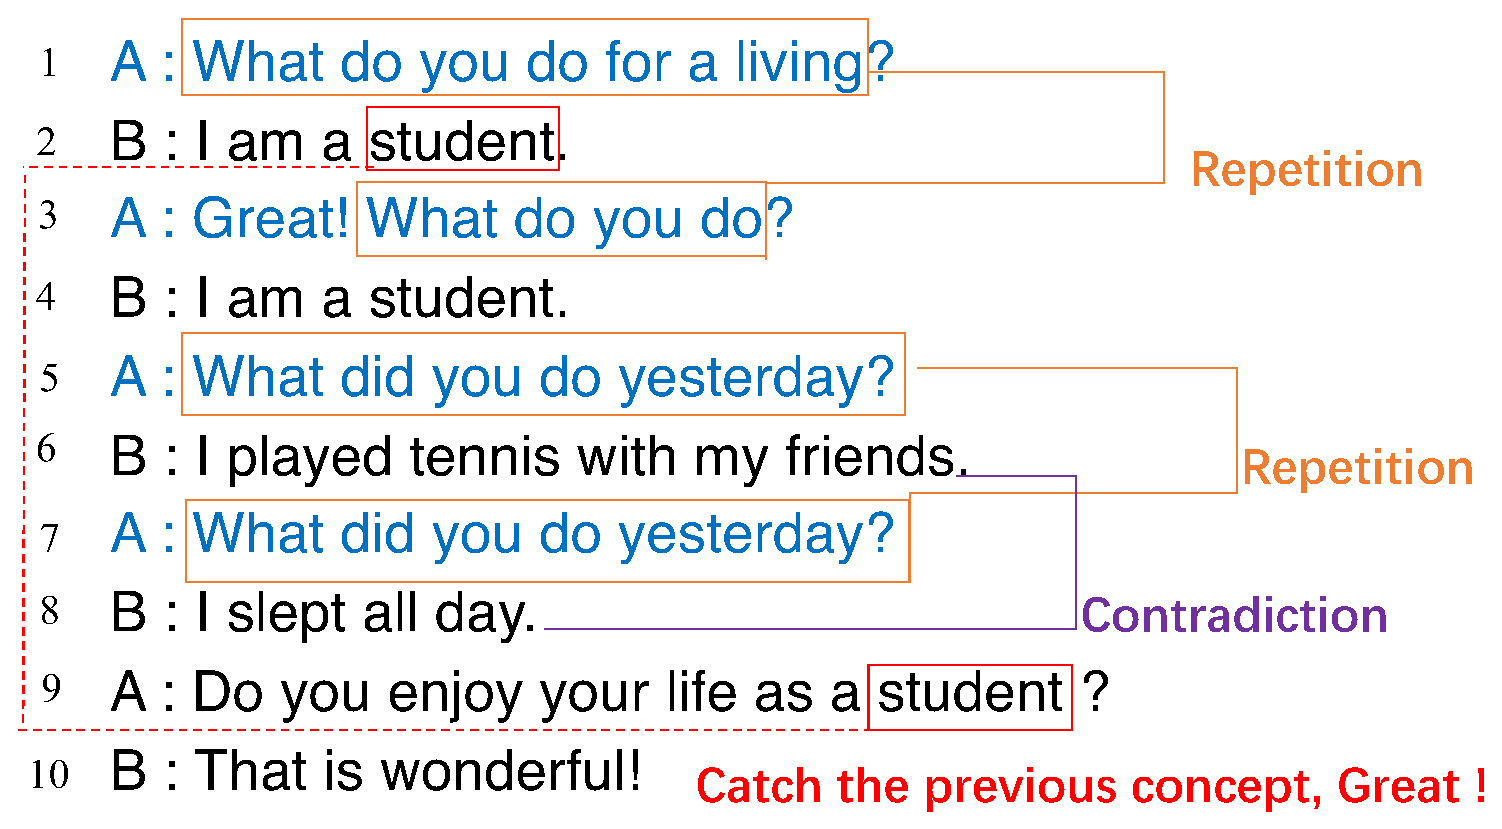
\includegraphics[width=0.95\columnwidth]{example.eps}
	\caption{An example snipet from a chat history between two bots.}
	\label{fig:example}
\end{figure}

The main contributions of this paper are as follows :
\begin{itemize}
\item We propose an interactive evaluation framework which allows chatbots 
to converse with each other directly and is modeled after 
the interaction of players in sports competitions (\ssecref{ssec:competition}).
\item  The entire scoring process is fully automated, saving 
time and manual effort. Given a number of bots to be evaluated, 
we can produce the ranking results in a minute (\ssecref{ssec:scoring}).
\item  Our experiments provide an example of the way to 
design a rule-based scoring system that closely tracks the 
human evaluation results. Preliminary results show
that our experimental chatbot evaluation system outperforms 
several recent strong baseline evaluation systems (\secref{sec:experiment}).
\end{itemize}
